\documentclass{article}
\usepackage[utf8]{inputenc}
\usepackage{graphicx}
\usepackage[left=2cm,right=2cm,top=2cm,bottom=2cm]{geometry}
\usepackage[frenchb]{babel}
\usepackage{float}


\begin{document}

\section{Kmeans}

\subsection{Influence du nombre de superpixel}

\begin{figure}[H]
\centering
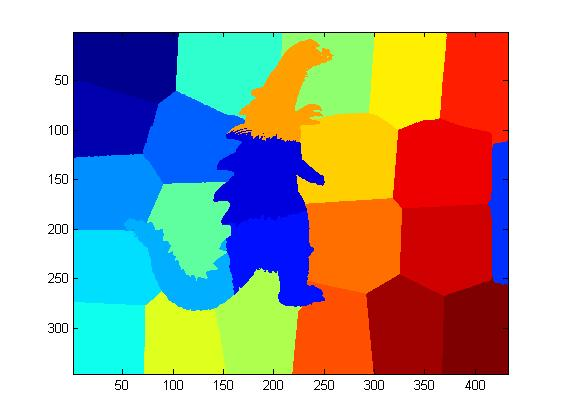
\includegraphics[width=0.49\textwidth]{kmeans25.jpg}
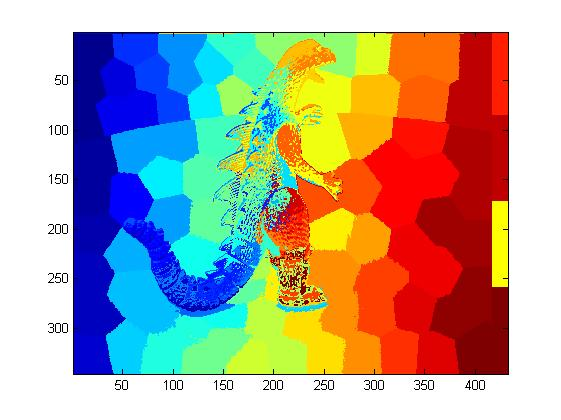
\includegraphics[width=0.49\textwidth]{kmeans144.jpg}
\caption{Influence du nombre de superpixel 25(gauche) 144(droite)}
\end{figure}

La diminution du nombre de superpixel permet de réduire le phénomène de sursegmentation mais certaine zone peuvent alors être mal segmenté. Dans l'exemple ci-dessus utilisant 25 superpixels les griffes, la machoire et les pattes du dinosaures sont mal segmentés.

\subsection{Influence du paramètre m de la distance utilisée}

L'utilisation d'une valeur élevé pour m permet de réduire le nombre de composante connexe dans l'image finale mais réduit l'importance de la distance colorimétrique dans la distance utilisée dans le kmeans. De plus un nombre élevé de coposante connexe n'est pas un problème car la suite de l'algorithme permet de corriger ce fait.

\begin{figure}[H]
\centering
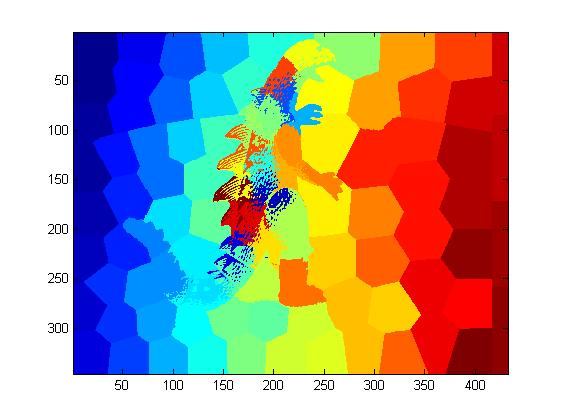
\includegraphics[width=0.49\textwidth]{m30.jpg}
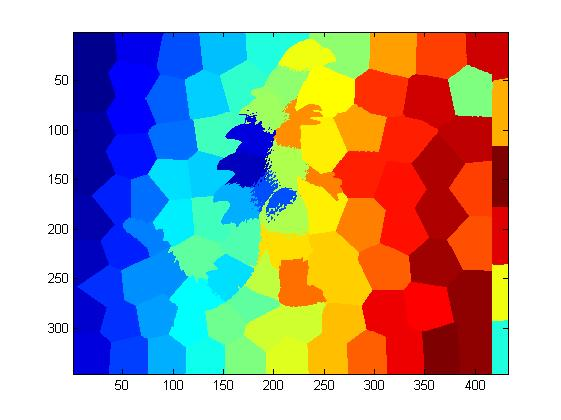
\includegraphics[width=0.49\textwidth]{m60.jpg}
\caption{Influence du paramètre m 30(gauche) 60(droite)}
\end{figure}

\section{Renforcement de la connéxité}

\subsection{Algorithme utilisé}

L'algorithme utilisé commencence par découper l'image en zone connexe en utilisant la 8-connéxité, ainsi à chaque pixel est associé un entier propre à la zone connexe à laquelle il appartient. Pour cela on utilise le vecteur idx obtenu par éxécution de l'algorithme kmeans, que l'on redimensionne sous forme d'une image. On applique alors bwlabel sur chaque classe.

Nous disposons maintenant d'une matrice d'entier de la taille de l'image dont le coéfficient $a_i_j$ identifie la composante connexe. La recherche des zones connexes adjacentes ainsi que la détermination du nombre de pixel composant la zone connexe en est alors aisé.

Le critère de fusion utilisé est la taille de la zone connexe. Si elle est inférieur à un pourcentage fixé de la taille moyenne d'un superpixel alors on fusionne la zone avec la composane connexe adjacente la plus grande.

\subsection{Influence du paramètre de fusion}

Dans l'illustration suivante chaque pixel a la couleur du centre auquel il appartient.

\begin{figure}[H]
\centering
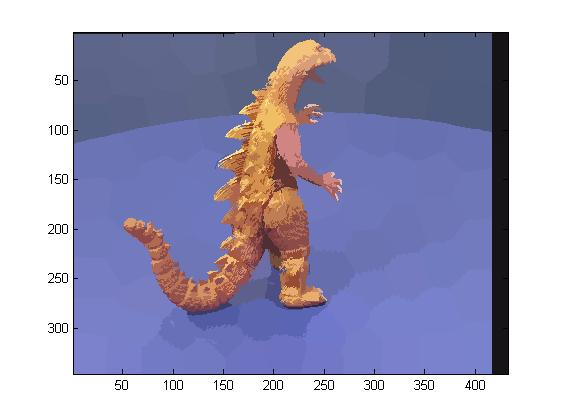
\includegraphics[width=0.49\textwidth]{renfconn001.jpg}
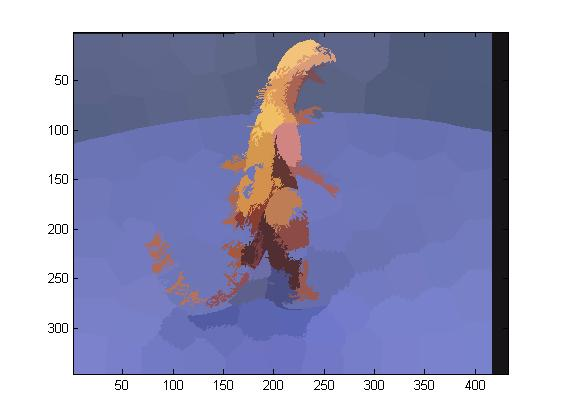
\includegraphics[width=0.49\textwidth]{renfconn02.jpg}
\caption{PourcentageFusion valant 1\% (à gauche) et 20\%(à droite)}
\end{figure}

On remarque qu'une fusion des zones connexes excessives peut provoquer le rattachement de certains pixels au fond de l'image. En effet dans l'image de droite ci dessus des parties de la queue du dinosaure ont été fusionné avec le fond de l'image.

Pour éviter un tel problème, il faudrait peut être changer le choix de la zone avec laquelle on fusionne. En effet plutot que de fusionner avec la plus grande zone adjacente il faudrait peut être fusionner avec la zone adjacente la plus proche d'un point de vue colorimétrique.

\section{Segmentation binaire}

La segmentation binaire se base sur l'application d'un seuil. Cependant il faut maintenant choisir sur quelles données appliquer le seuillage. Nous avons choisi d'appliquer ce seuil sur la composante rouge de l'image segmentée. En effet l'image représentant un dinosaure à dominante rouge sur fond à dominante bleue, ce choix nous a paru légitime et génère de bons résultats.

\begin{figure}[H]
\centering
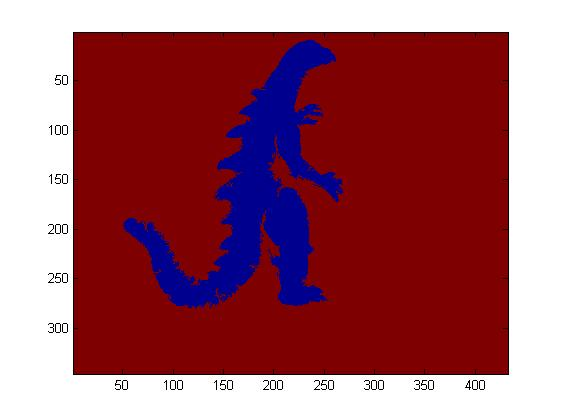
\includegraphics[width=0.8\textwidth]{bin.jpg}
\caption{Résultat de la segmentation binaire}
\end{figure}

\end{document}